\documentclass{article}

\usepackage{graphicx}
\usepackage{tikz}
\usepackage{tikzsymbols}
\usetikzlibrary{calc,patterns,shapes.geometric}
\pagestyle{empty}
\usepackage[margin=0pt]{geometry}
\geometry{papersize={14in,12in}}

\def\centerarc[#1](#2)(#3:#4:#5){\draw[#1] ($(#2)+({#5*cos(#3)},{#5*sin(#3)})$) arc (#3:#4:#5);}

\begin{document}
	\begin{figure}
		\centering
		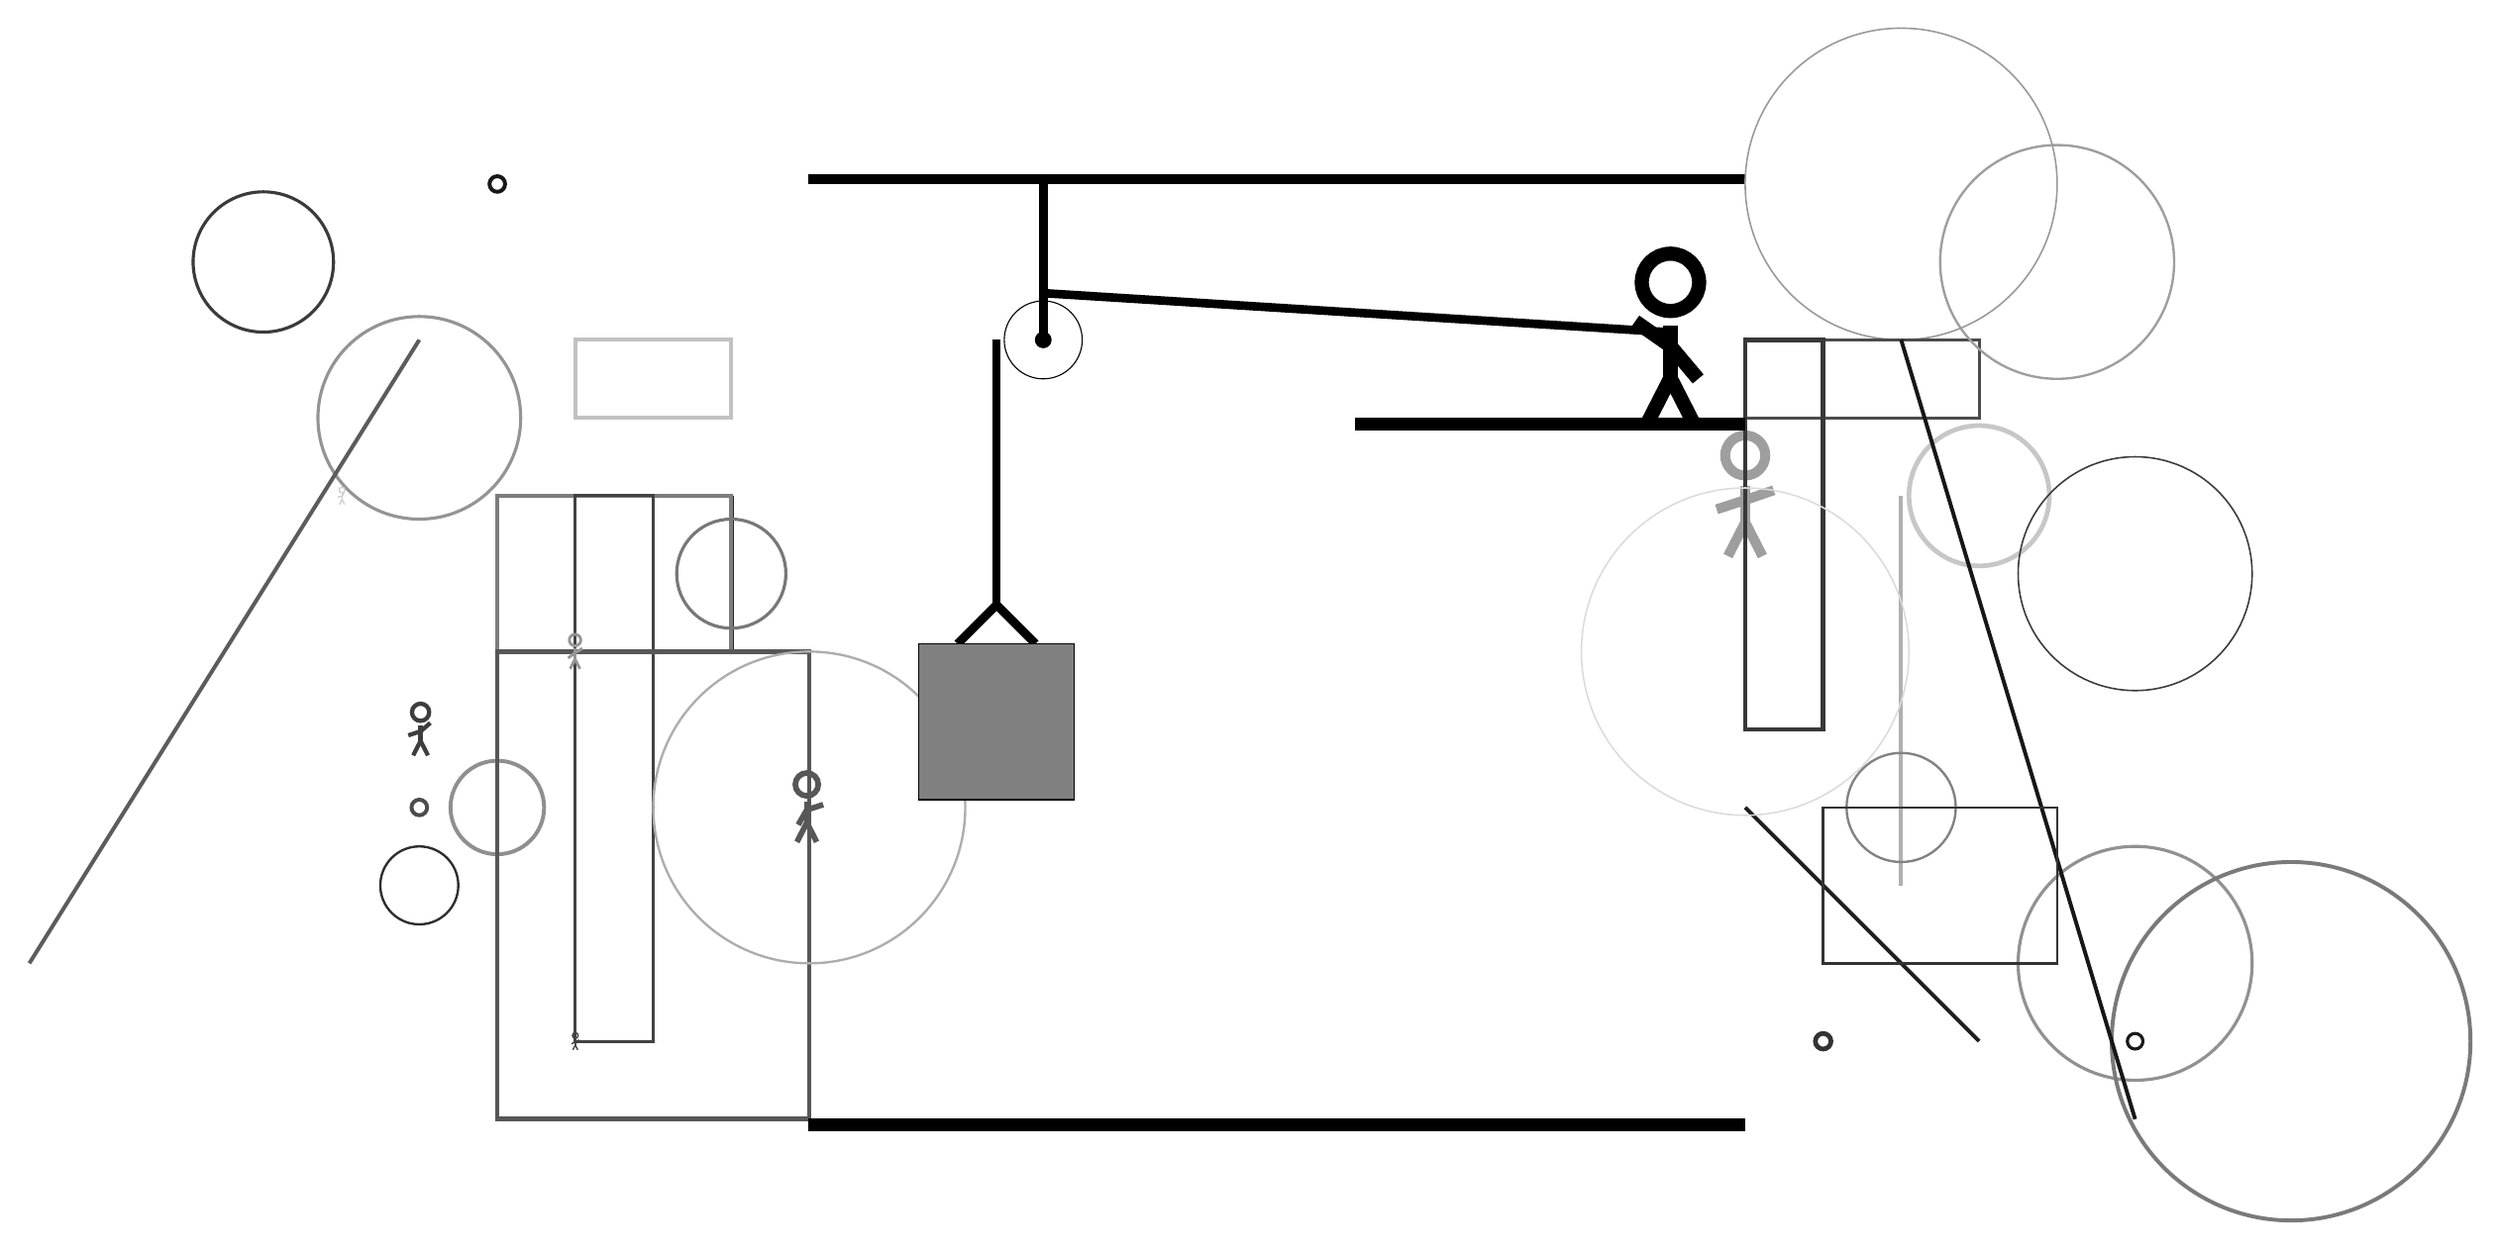
\begin{tikzpicture}
			%%%%% START %%%%%
			
			\draw[fill=black] (-2, 9) rectangle (10, 9.125);
			
			\draw (1, 7) circle (0.5);
			\draw[fill=black] (1, 7) circle (0.1);
			\draw[line width=1.1mm] (1, 9) -- (1, 7);
			
			\draw [line width=0.4mm, color=black!43](15, -1) circle (1.5);
			
			\draw[line width=0.7mm, color=black!10] (11, 6) rectangle (11, 4);
			\draw [line width=0.5mm, color=black!91](-6, 9) circle (0.1);
			\draw[line width=0.7mm, color=black!84] (-3, 5) rectangle (-3, 3);
			\draw [line width=0.4mm, color=black!42](-7, 6) circle (1.3);
			\draw[line width=0.5mm, color=black!51] (-3, 3) rectangle (-6, 5);
			\draw [line width=0.4mm, color=black!77](-9, 8) circle (0.9);
			
			\draw [line width=0.3mm, color=black!82](-7, 0) circle (0.5);
			\node[line width=0.4mm, color=black!71] at (-5, -2) {\Strichmaxerl[1][27][27]};
			
			\draw [line width=0.2mm, color=black!40](12, 9) circle (2.0);
			
			\draw[line width=0.5mm, color=black!64](-7, 7) -- (-12, -1);
			\draw [line width=0.5mm, color=black!44](-6, 1) circle (0.6);
			\draw[line width=0.5mm, color=black!88](13, -2) -- (10, 1);
			\draw [line width=0.4mm, color=black!53](-3, 4) circle (0.7);
			\node[line width=0.2mm, color=black!66] at (-2, 1) {\Strichmaxerl[4][60][18]};
			\draw[line width=0.4mm, color=black!74] (-4, 5) rectangle (-5, -2);
			\draw[line width=0.6mm, color=black!66] (-2, -3) rectangle (-6, 3);
			\draw [line width=0.6mm, color=black!22](13, 5) circle (0.9);
			\draw [line width=0.5mm, color=black!70](-7, 1) circle (0.1);
			\draw[line width=0.5mm, color=black!24] (-3, 7) rectangle (-5, 6);
			\draw [line width=0.5mm, color=black!52](17, -2) circle (2.3);
			
			\draw[line width=0.4mm, color=black!70] (10, 7) rectangle (13, 6);
			\draw[line width=0.5mm, color=black!31](12, 5) -- (12, 0);
			\draw[line width=0.5mm, color=black!91](15, -3) -- (12, 7);
			\draw [line width=0.3mm, color=black!32](-2, 1) circle (2.0);
			\draw [line width=0.6mm, color=black!80](11, -2) circle (0.1);
			
			\draw [line width=0.3mm, color=black!49](12, 1) circle (0.7);
			\draw[line width=0.4mm, color=black!87] (10, 0) rectangle (10, 0);
			\node[line width=0.7mm, color=black!41] at (-5, 3) {\Strichmaxerl[2][37][31]};
			
			\node[line width=0.3mm, color=black!76] at (-7, 2) {\Strichmaxerl[3][18][41]};
			\node[line width=0.7mm, color=black!38] at (10, 5) {\Strichmaxerl[7][18][19]};
			
			\draw [line width=0.2mm, color=black!77](15, 4) circle (1.5);
			\draw[line width=0.3mm, color=black!80] (11, 1) rectangle (14, -1);
			
			\draw [line width=0.3mm, color=black!38](14, 8) circle (1.5);
			\draw[line width=0.6mm, color=black!78] (10, 2) rectangle (11, 7);
			\draw [line width=0.4mm, color=black!90](15, -2) circle (0.1);
			
			\node[line width=0.4mm, color=black!19] at (-8, 5) {\Strichmaxerl[1][10][62]};
			
			\draw [line width=0.2mm, color=black!14](10, 3) circle (2.1);
			
			\draw[line width=1.1mm](-0.1, 3.1) --  (0.4, 3.6) -- (0.9, 3.1);
			\draw[fill=black!50] (-0.6, 3.1) rectangle (1.4, 1.1);
			
			\draw[line width=1.1mm](0.4, 7) -- (0.4, 3.6);
			\centerarc[line width=1.1mm](1, 7)(90:180:0.6)
			\draw[line width=1.1mm](1, 7.6) -- (9, 7.1);
			
			\node at (9, 7) {\Strichmaxerl[10][-35][-50]};
			\draw[fill=black] (5, 6) rectangle (10, 5.85);
			
			\draw[fill=black] (-2, -3) rectangle (10, -3.15);
			
			%%%%% END %%%%%
		\end{tikzpicture}
	\end{figure}	
\end{document}